\section{Presentation Logic Layer}

%What pages will be present in your project? briefly indicate how your web site will be organized

Here are listed the main pages that will be available on our web application:

\begin{itemize}
    \item Login Page: here the user can log in filling the form with his username and password;
    \item Home Page: the home page of the application: the home page will be reached immediately after the login part. Here some of the insight plots will be displayed. on the left side of the page a nav menu will be shown, with the dropdown menu that will allow to choose the current company used, and all other following sections will be displayed as links;
    \item User Page: here the user can access to his reserved area, in which will able to modify user settings, notification settings, company settings and bank account settings through forms;
    \item Product Creation Page: here the user will have a form to insert a new product in the database;
    \item Product Update Page: here the user will have firstly the possibility to choose one of his products through a radio button: once one is chosen, he will be redirected to a pre-filled form of the product, in which he will be able to modify it;
    \item Product Delete Page: here the user will have the possibility to delete a product, through a radio button;
    \item Product List Page: here a list of all products will be listed: a button will allow the user to download in pdf format a list of all the products;
    \item Customer Creation Page: here the user will have a form to insert a new customer in the database;
    \item Customer Update Page: here the user will have firstly the possibility to choose one of his customers through a radio button: once one is chosen, he will be redirected to a pre-filled form of the customer, in which he will be able to modify it;
    \item Customer Delete Page: here the user will have the possibility to delete a customer, through a radio button;
    \item Customer List Page: here a list of all customers will be listed: a button will allow the user to download in pdf format a list of all the customers;
    \item Invoice Creation Page: here a new invoice entity will be created, setting up some general data through a form, as for example to which customer the invoice will be related;
    \item Invoice Update Page: here the user can edit the data entered in the creation part;
    \item Invoice List Page: here the user can look to the list of his invoices, in which he will see all the open invoices, in which he will able to add invoice rows, closed invoices that are waiting to be billed (invoice warning PDF will be available for download), and billed invoices (actual invoice in both PDF and XML will be available for download). Filters to the list will be available.
    \item Invoice Row List Page: by clicking on an invoice a list of all invoice rows of a specific invoice will be available;
    \item Invoice Row Insertion Page: by clicking on a specific button on open invoices, a form to insert a new row on the invoice will be available, in which also the product sold will be available;
    \item Detailed Insights Page: a page where the user can see all the insights available.
\end{itemize}
\newpage


\subsection{Login page - Reset password page - New password page}

\begin{itemize}
    \item \textbf{Login page}: Through the log-in page, users can access the restricted area in which they can manage their companies' electronic invoicing. To access, it is necessary to enter e-mail and password in the appropriate fields and click on the "Log-in" button.
In case the user has forgotten his password, he can click on the "Reset here" button to set a new one.
    \item \textbf{Reset password page}: On this page you can make a request to reset the password. Once the e-mail is entered and "Send e-mail" is clicked, the user will be emailed a link to enter the new password. Clicking "Cancel" will return the user to the Login page.
    \item \textbf{New password page}: The user must enter the new password twice in the appropriate fields and click on "Confirm reset" to set the new password. Clicking on "Cancel" will return to the Login page.
\end{itemize}

\begin{figure}[h!]
    \centering
    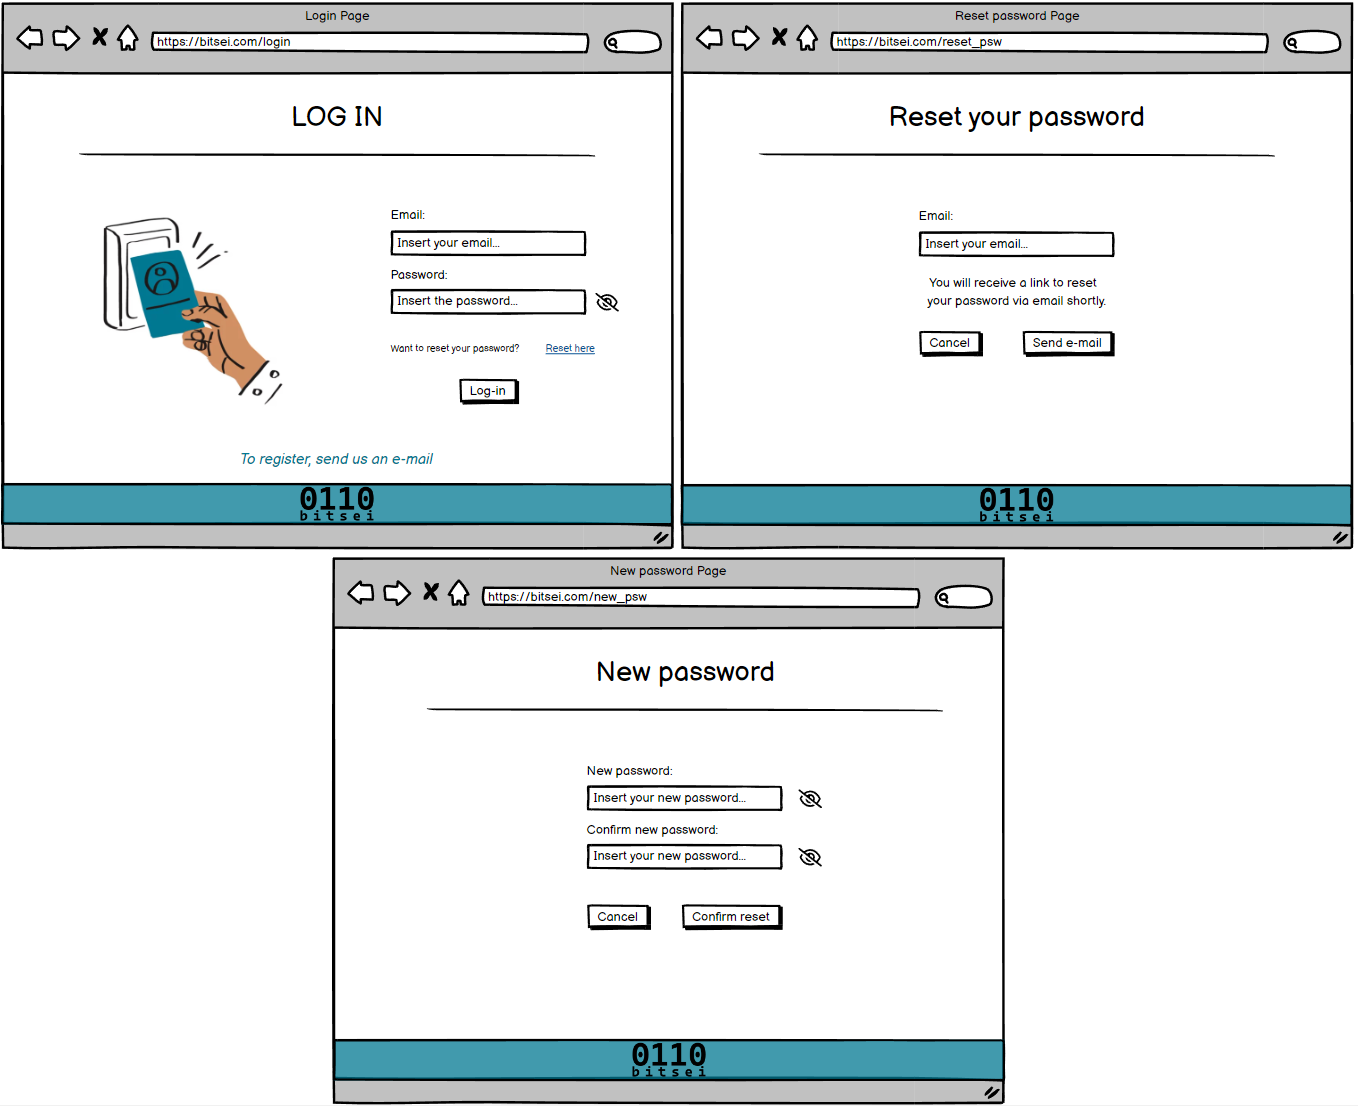
\includegraphics[height=390pt, keepaspectratio]{resources/mockup/Login.png}
\end{figure}
\newpage

\subsection{Home page}
The home page will be reached immediately after the login part. Here some of the insight plots will be displayed. On the left side of the page a nav menu will be shown. In the upper right corner there is a dropdown menu to choose the desired company.
\begin{figure}[h!]
    \centering
    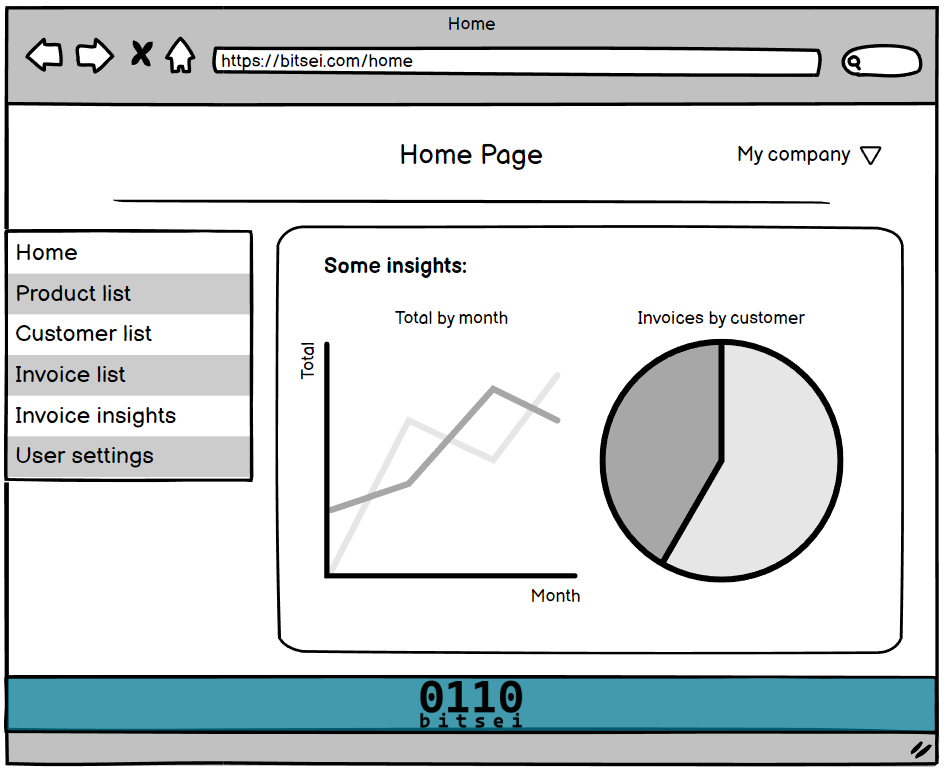
\includegraphics[height=380pt, keepaspectratio]{resources/mockup/Home.png}
\end{figure}
\newpage
\subsection{Invoice list page}
This page shows all invoices related to your company. \\
On the right side you can set some filters for searching. You can filter invoices by: total, discount, date, warning date, pfr, customer, product. To activate a filter you need to click on the switch next to it.\\
In the list, each invoice is displayed with an identifier and other information to make searching easier. Clicking above the invoice will take you to the "Inovice details" page that allows you to view information regarding the invoice. Above each item in the list are 3 buttons: edit, edit rows, and delete. The first two lead to the respective dedicated pages. the last one is used to delete an invoice (when clicked, a pop-up is shown to confirm the deletion). These buttons are clickable only if the invoice has not reached the "Closed" status. Finally, in the list, there is a button to create a new invoice that leads to the "Create invoice" page.\\
In the upper right is an input field to search for the desired invoice.\\
The bottom left shows the number of invoices resulting from the search. In the lower center corner you can choose how many invoices to display (by default all are displayed). Finally, at the top center, via a menu, you can choose in what order to display the invoices.\\
\begin{figure}[h!]
    \centering
    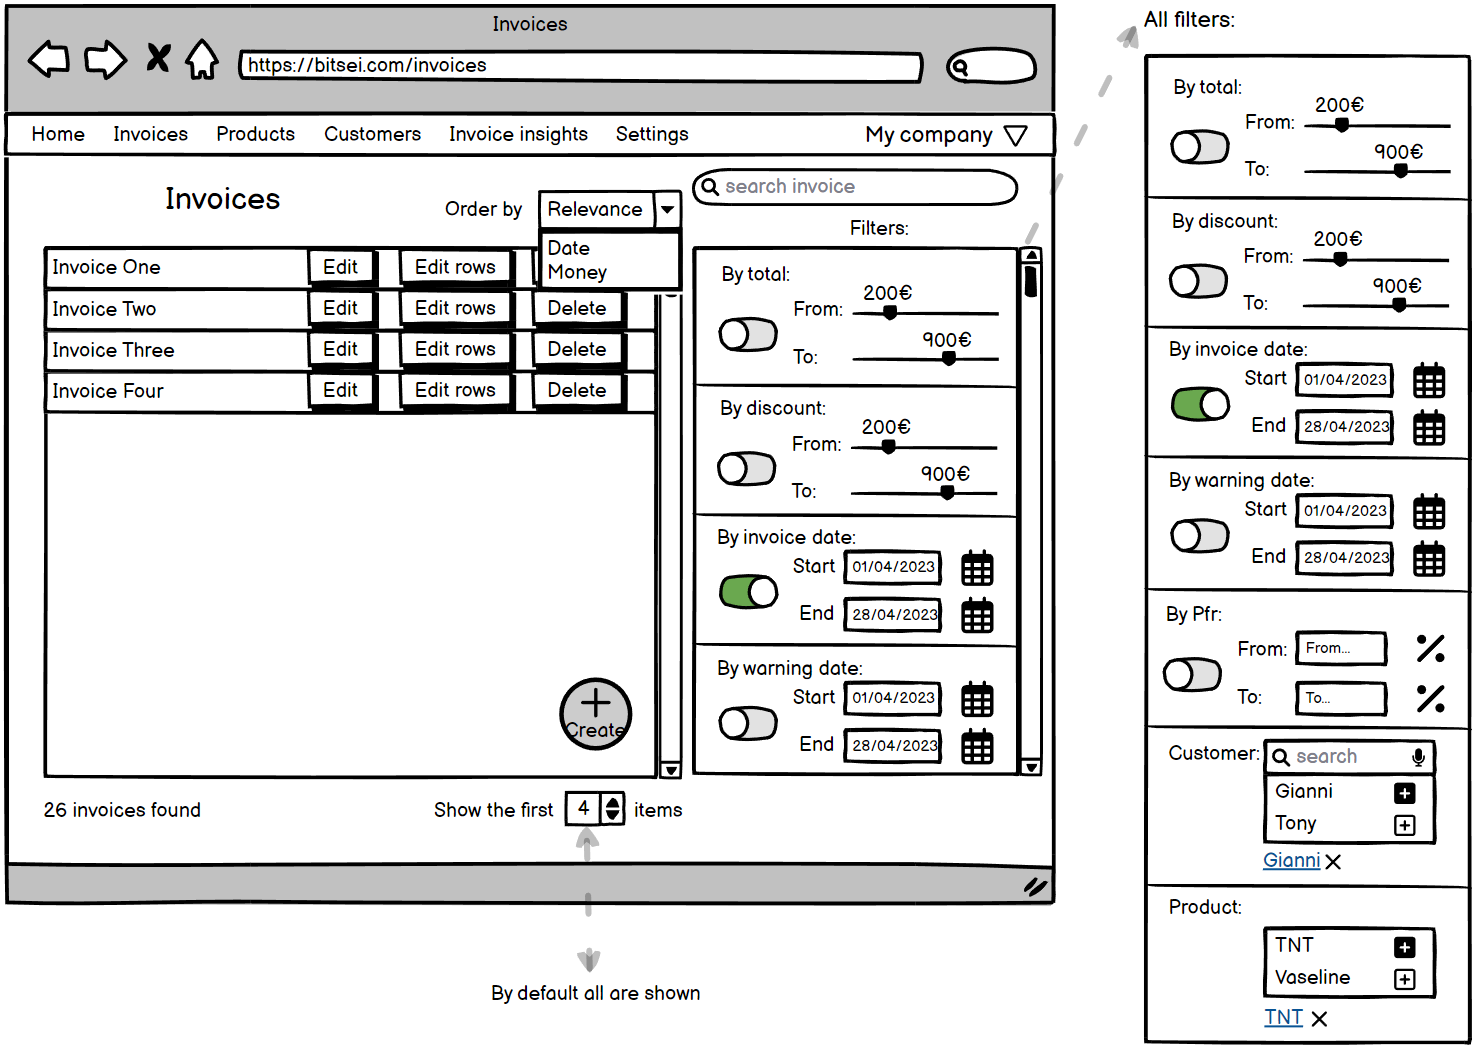
\includegraphics[height=350pt, keepaspectratio]{resources/mockup/Invoice_list.png}
\end{figure}
\newpage

\subsection{Create invoice page - Edit invoice page - Invoice rows page}

\begin{itemize}
    \item \textbf{Create invoice page}: On this page you can create a new invoice. At the top are fields to be filled in, and at the bottom is the table displaying all rows related to this invoice. To add or edit rows you need to click on the "Edit rows here" link that leads to the "Edit rows" page. Still further down are two buttons, one to cancel and return to the invoice list and one to confirm the creation of the invoice.
    \item \textbf{Edit invoice page}: This page is similar to the invoice creation page only it refers to an invoice that has already been created previously. In this case the fields are already filled with the previous values. At the bottom there are two buttons, one to cancel and return to the "Invoice list" page and one to save the changes.
    \item \textbf{Invoice rows page}: A table containing all rows concerning the invoice is displayed. Each cell in the table can be edited by double-clicking on it. Using check-boxes, various invoices can be selected and then deleted using the "Delete" button. There is a button in the table to add a new row (Initially it will be filled with default values). Finally there is a button to return to the previous page.
\end{itemize}

\begin{figure}[h!]
    \centering
    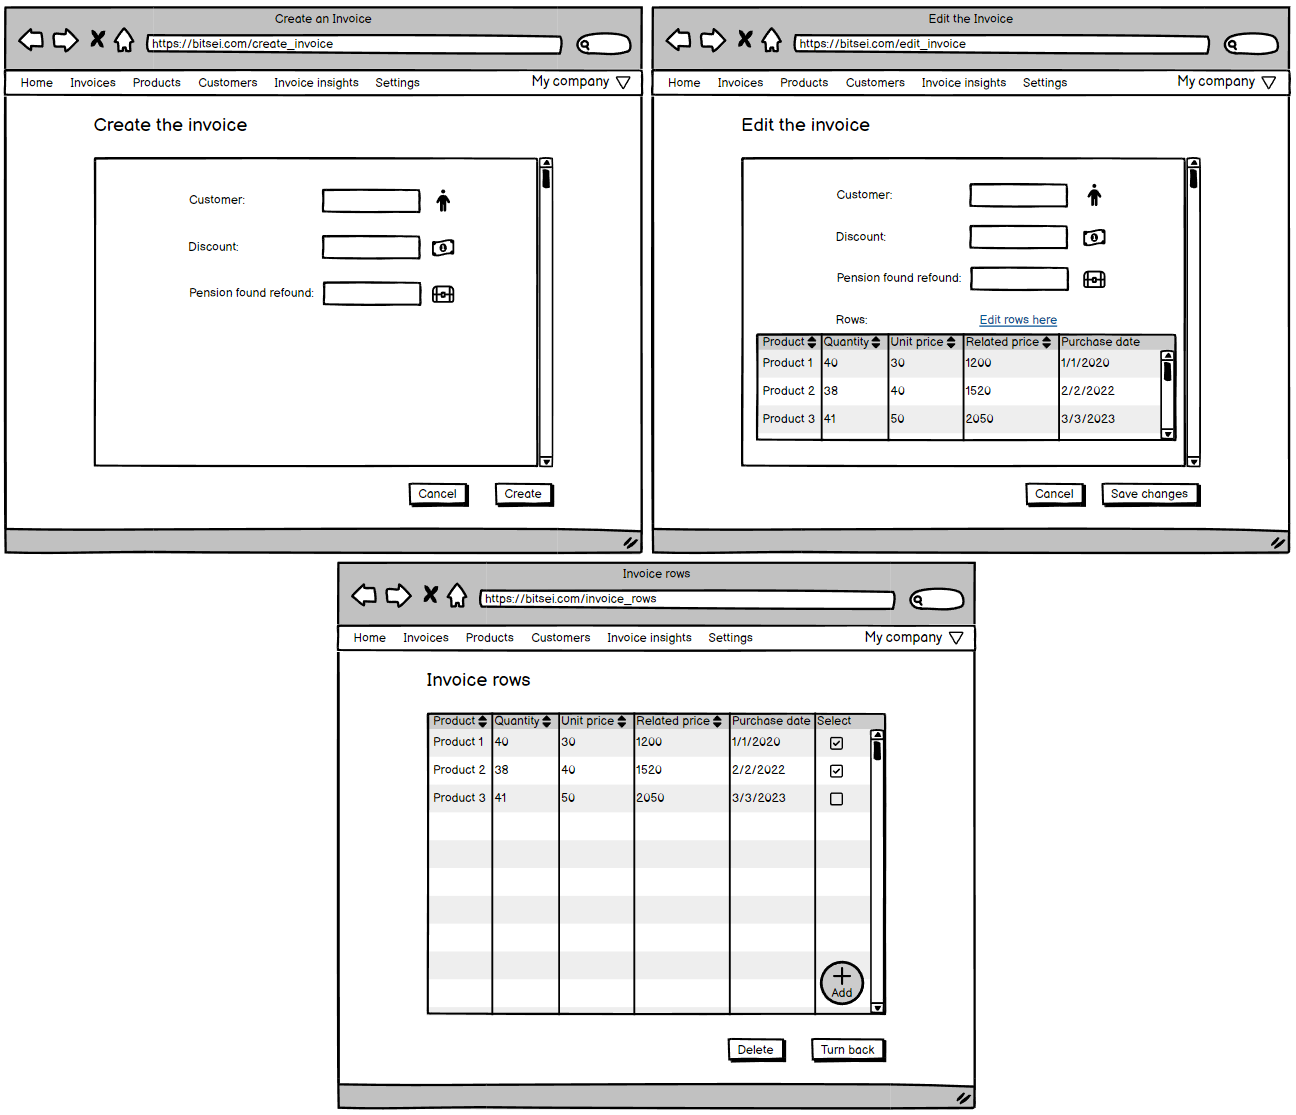
\includegraphics[height=410pt, keepaspectratio]{resources/mockup/Invoice.png}
\end{figure}
\newpage

\subsection{Invoice details page}
On this page you can view all the details of an invoice. The fields cannot be edited. At the bottom is a label indicating the status of the invoice (can be Created, Closed, Completed). Then there are buttons to: edit rows, edit the invoice, delete the invoice. These buttons are only available if the status is "Created". By clicking on "Delete" a pop-up is shown to confirm the deletion. Finally there is a button to return to the previous page.
At the top right are two buttons, one for downloading the invoice document and the other for exporting it via email. These buttons are disabled in the "Created" state, in the "Closed" state only the invoice notice will be downloaded. In the "Completed" state you will be able to choose whether to download the invoice notice or the invoice in either pdf or xml format.
\begin{figure}[h!]
    \centering
    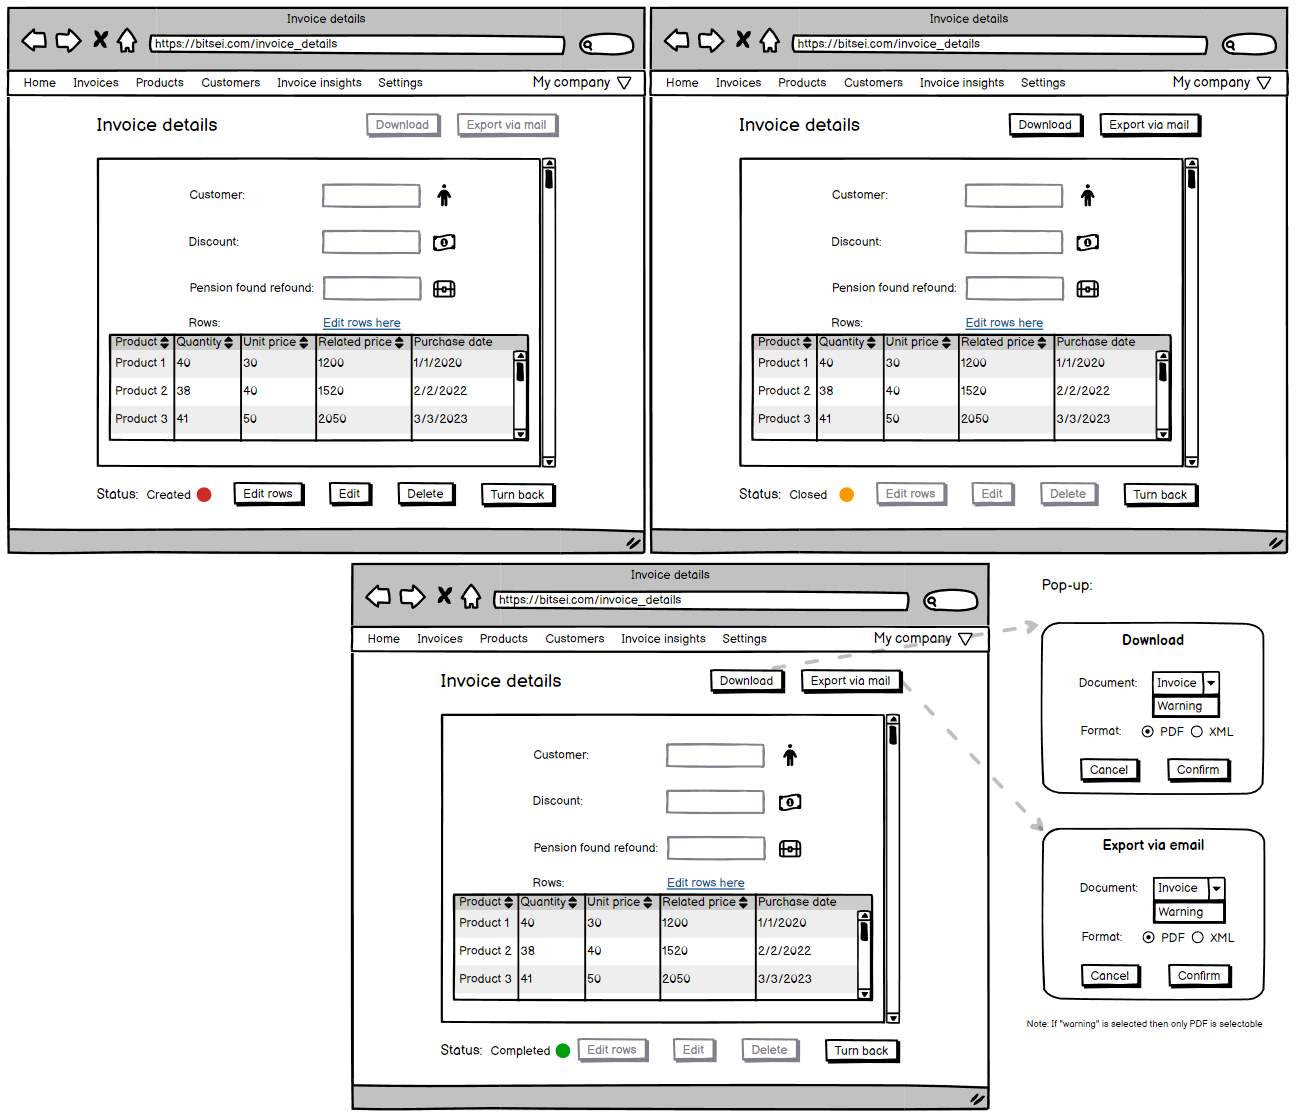
\includegraphics[height=410pt, keepaspectratio]{resources/mockup/Invoice_details.png}
\end{figure}
\newpage

\subsection{Invoice insights page}
On this page you can view some charts related to your company. The charts available are: invoices by date, total by date, discount by date, invoices by customer, total by customer. It is possible to change graphs by selecting the desired one in the menu tab. Dates in the x-axis can be grouped by month, day, year. Filters can be applied on the right so that only certain elements are taken into account. At the top right are two buttons for downloading and exporting the chart by e-mail.
\begin{figure}[h!]
    \centering
    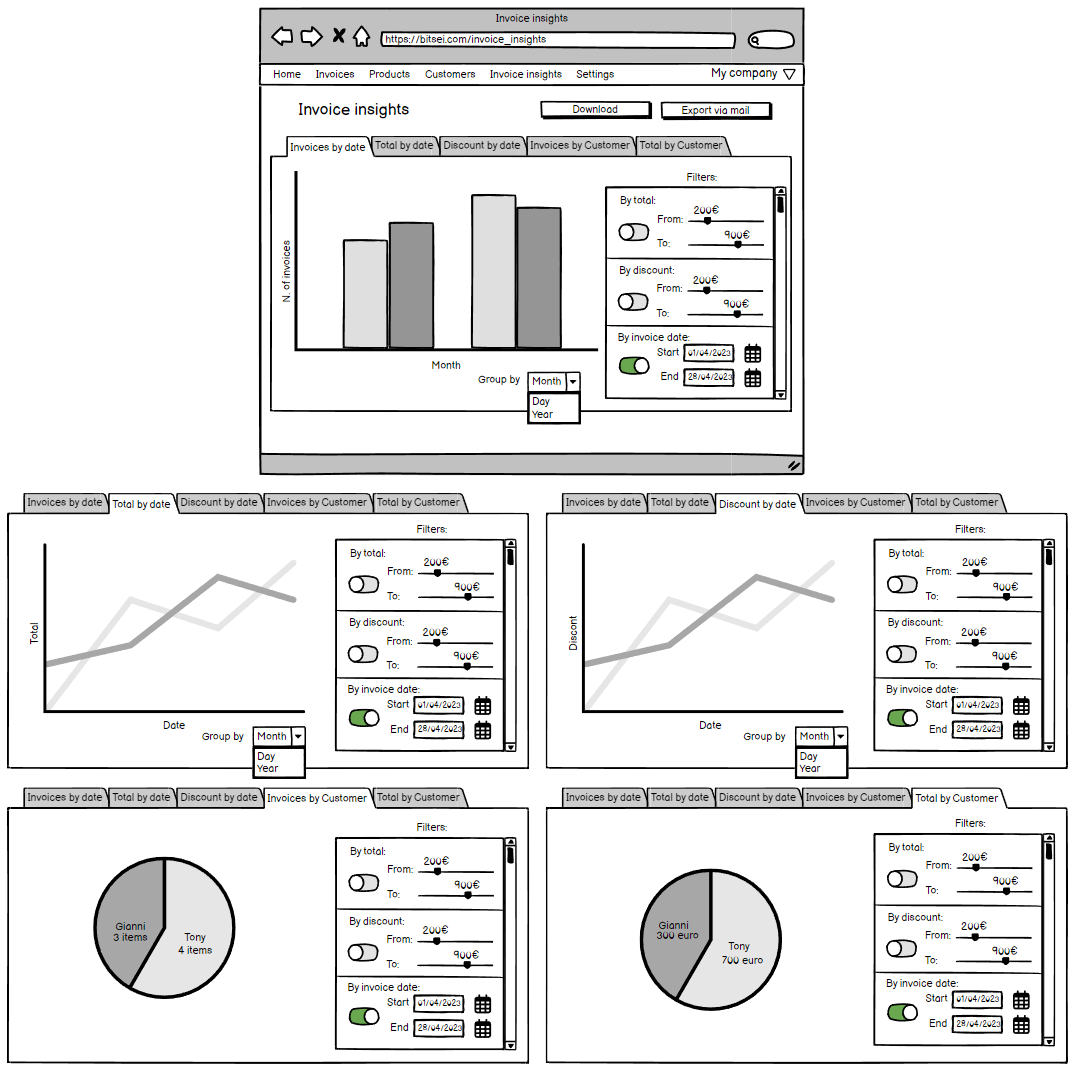
\includegraphics[height=460pt, keepaspectratio]{resources/mockup/Invoice_insights.png}
\end{figure}
\newpage

\subsection{Product list page - Create product page - Product details page - Edit product page}

\begin{itemize}
    \item \textbf{Product list page}: This page shows all products related to your company.
In the list, each product is displayed with his name. Clicking above the product will take you to the "Product details" page that allows you to view information regarding the product. Above each item in the list are 2 buttons: edit, and delete. The first lead to the dedicated page. The second one is used to delete a product (when clicked, a pop-up is shown to confirm the deletion). In the list, there is a button to add a new product that leads to the "Create product" page.
In the upper right is an input field to search for the desired product.
The bottom left shows the number of products resulting from the search. In the lower right corner you can choose how many products to display (by default all are displayed). Finally, at the top center, via a menu, you can choose in what order to display the products.
At the bottom center are two buttons, one for downloading the product list summary and the other for exporting it via email.
    \item \textbf{Create product page}: On this page you can add a new product. There are fields to be filled in. Still further down are two buttons, one to cancel and return to the product list and one to confirm the addition of the product.
    \item \textbf{Product details page}: On this page you can view all the details of a product. The fields cannot be edited. At the bottom there are buttons to: edit the product, delete the product. By clicking on "Delete" a pop-up is shown to confirm the deletion. Finally there is a button to return to the previous page.
    \item \textbf{Edit product page}: This page is similar to the product creation page only it refers to a product that has already been added previously. In this case the fields are already filled with the previous values. At the bottom there are two buttons, one to cancel and return to the "Product list" page and one to save the changes.
\end{itemize}
\newpage
\begin{figure}[h!]
    \centering
    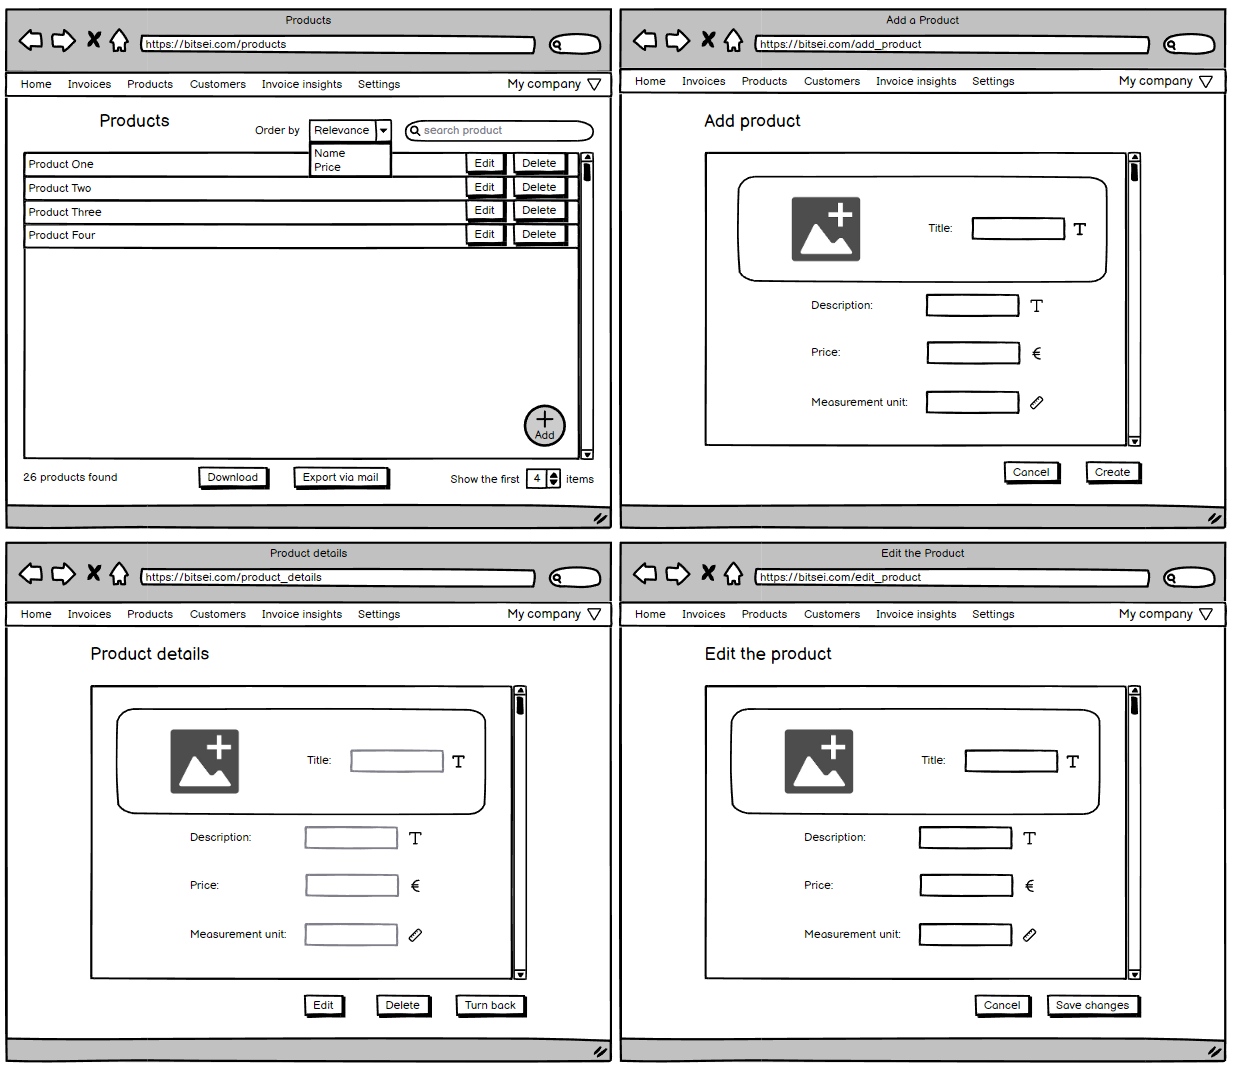
\includegraphics[height=420pt, keepaspectratio]{resources/mockup/Product.png}
\end{figure}
\newpage

\subsection{Customer list page - Create customer page - Customer details page - Edit customer page}

\begin{itemize}
    \item \textbf{Customer list page}: This page shows all customers related to your company.
In the list, each customer is displayed with his name. Clicking above the customer will take you to the "Customer details" page that allows you to view information regarding the customer. Above each item in the list are 2 buttons: edit, and delete. The first lead to the dedicated page. The second one is used to delete a customer (when clicked, a pop-up is shown to confirm the deletion). In the list, there is a button to add a new customer that leads to the "Create customer" page.
In the upper right is an input field to search for the desired customer.
The bottom left shows the number of customers resulting from the search. In the lower right corner you can choose how many customers to display (by default all are displayed). Finally, at the top center, via a menu, you can choose in what order to display the customers.
At the bottom center are two buttons, one for downloading the customer list summary and the other for exporting it via email.
    \item \textbf{Create customer page}: On this page you can add a new customer. There are fields to be filled in.At the bottom are two buttons, one to cancel and return to the customer list and one to confirm the addition of the customer.
    \item \textbf{Customer details page}: On this page you can view all the details of a customer. The fields cannot be edited. At the bottom there are buttons to: edit the customer, delete the customer. By clicking on "Delete" a pop-up is shown to confirm the deletion. Finally there is a button to return to the previous page.
    \item \textbf{Edit customer page}: This page is similar to the customer creation page only it refers to a customer that has already been added previously. In this case the fields are already filled with the previous values. At the bottom there are two buttons, one to cancel and return to the "Customer list" page and one to save the changes.
\end{itemize}
\newpage
\begin{figure}[h!]
    \centering
    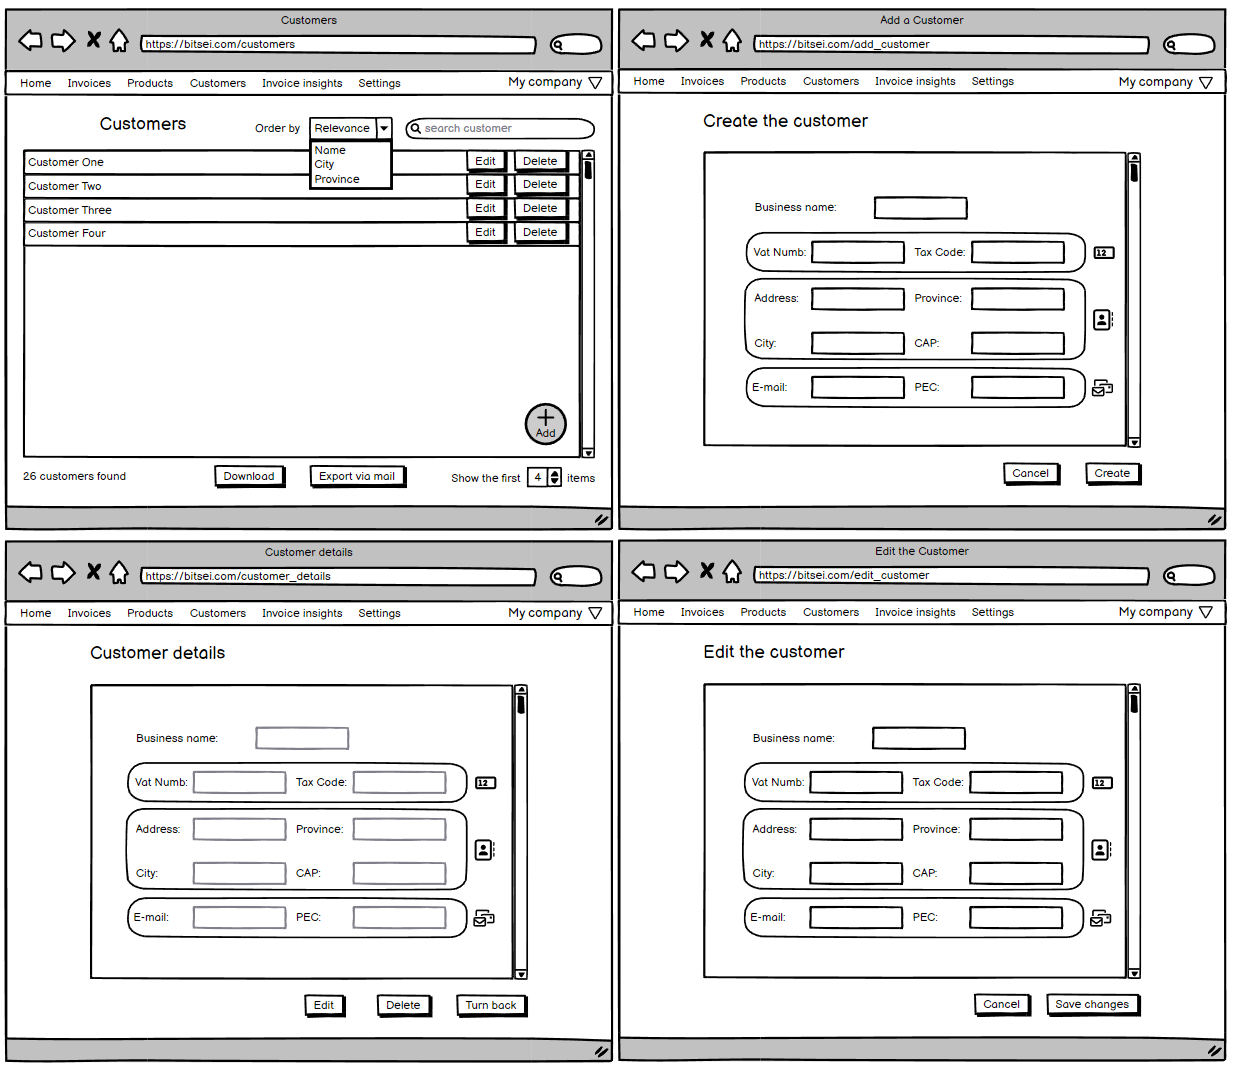
\includegraphics[height=420pt, keepaspectratio]{resources/mockup/Customer.png}
\end{figure}
\newpage

\subsection{Settings page}
This page is divided in two sections: Company settings and Bank Accunt settings. In the first one you can view or edit all the informations regarding your company. In the second one you can manage your bank accounts.
In the company section the fields are already filled with the previous values, in the bank account settings, the accounts are represented in a table.
If you want to change something at the end you need to click into "Save changes", otherwise you can click on "Cancel" to return back.
\begin{figure}[h!]
    \centering
    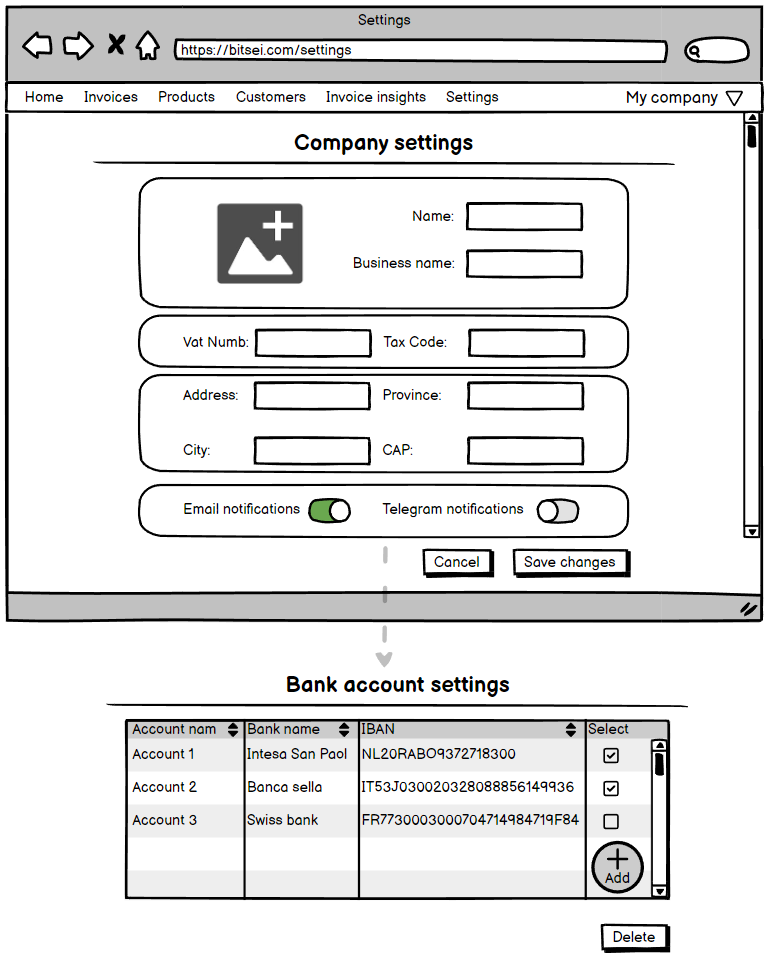
\includegraphics[height=530pt, keepaspectratio]{resources/mockup/Settings.png}
\end{figure}